\subsection{premi/client/frameEditor}
\begin{figure}[h]
\begin{center}
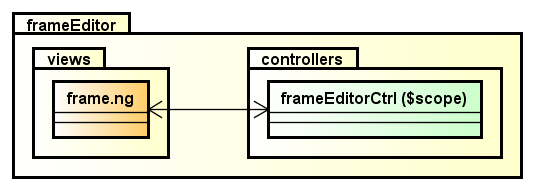
\includegraphics[scale=0.90]{img/diapkg/frameEditor.png}
\caption{Diagramma del package premi/client/frameEditor}
\end{center}
\end{figure}








%-------  diagramma della classe%
\subsubsection{premi/client/frameEditor/controllers/frameEditorCtrl}
\begin{figure}[h]
\begin{center}
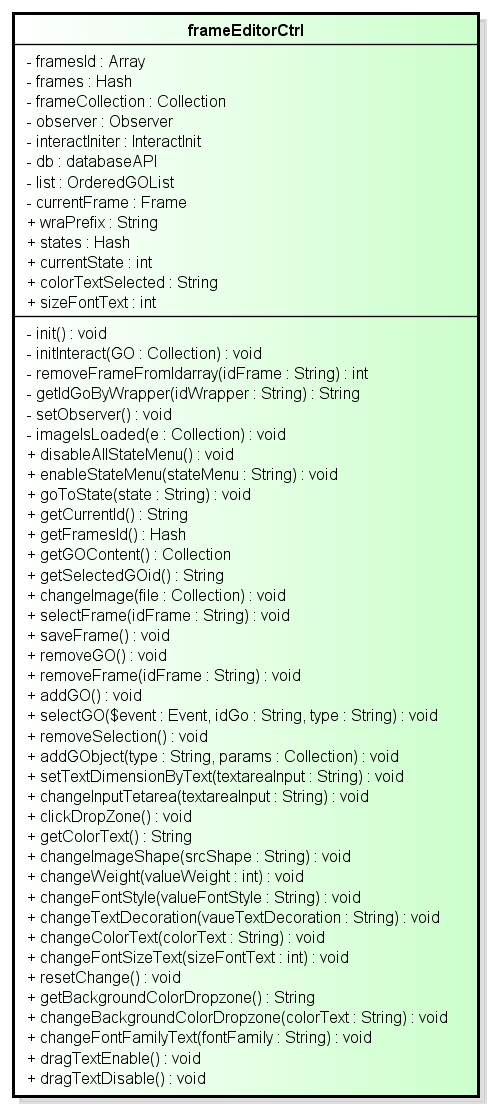
\includegraphics[scale=0.90]{img/diacla/frameEditorCtrl.png}
\caption{Diagramma della classe premi/client/frameEditor/controllers/frameEditorCtrl}
\end{center}
\end{figure}


\begin{description}
%-------  descrizione della classe%
\item[Descrizione] \hfill \\
	Questo controller crea lo \$scope associato alla vista generata da \textbf{frame.ng}, fornendo i dati e i metodi necessari per consentire all'utente di creare e modellare un frame, inserendo o rimuovendo oggetti grafici al suo interno.
	
	
%-------  lista delle classi associate%	
\item[Dipendenze] \hfill \\
	\begin{itemize}
		\item \textbf{premi/client/presentation/lib/OrderedGoList}: per la gestione degli oggetti grafici contenuti nei frame
		\item \textbf{premi/client/presentation/lib/databaseAPI}: per il salvataggio dei frame nel database
		\item \textbf{premi/client/editor/lib/InteractInit}: per accedere alla libreria Interact.JS e offrire una rappresentazione grafica dei frame all'utente
		\item \textbf{premi/client/editor/lib/Frame}: per la creazione e la modifica dei frame
		\item \textbf{premi/client/editor/lib/Observer}: per dare un Observer agli oggetti che ne fanno uso
	\end{itemize}
	
	
%-------  lista degli Attributi%	
\item[Attributi] \hfill \\
	\begin{description}
		\item[\textbf{- framesId : Array			}] \hfill \\
			Array dei codici identificativi dei frame creati dall'utente nella presentazione che sta modificando
		\item[\textbf{- frames : Hash			}] \hfill \\
			Hash dei frames creati dall'utente in questa presentazione, strutturato come \textit{id\_frame} : \textit{Collezione JSON dei suoi attributi}
		\item[\textbf{- frameCollection : Collection			}] \hfill \\
			Collezione di MongoDB dei frames contenuti nella presentazione che l'utente sta modificando
		\item[\textbf{- observer : Observer			}] \hfill \\
			Observer della classe, che andrà associato agli oggetti con cui l'utente lavora
		\item[\textbf{- interactIniter : InteractInit			}] \hfill \\
			interactIniter è utilizzato per l'inizializzazione della libreria Interact.JS
		\item[\textbf{- db : databaseAPI			}] \hfill \\
			Contiene una lista di metodi coi quali la classe può salvare i dati dell'utente nel database
		\item[\textbf{- list : OrderedGOList			}] \hfill \\
			È la lista di oggetti grafici contenuti nel frame che l'utente sta modificando
		\item[\textbf{- currentFrame : Frame			}] \hfill \\
			È il frame che l'utente sta modificando
		\item[\textbf{+ wraPrefix : String			}] \hfill \\
			Stringa che indica quale prefisso si sta utilizzando per gli oggetti "wrapper" che compongono l'interfaccia grafica di questa parte di editor
		\item[\textbf{+ states : Hash			}] \hfill \\
			Oggetto contenente una lista di stati che l'editor può assumere durante il suo utilizzo da parte dell'utente. Una volta inizializzato non può più essere modificato. Inizializzarlo con i seguenti campi:
		\begin{itemize}
			\item noSelection : 1
			\item imageEditing : 2
			\item shapeEditing : 3
			\item textEditing : 4
			\item addingGo : 5
			\item framesList : 6
		\end{itemize}
		\item[\textbf{+ currentState : int			}] \hfill \\
			Lo stato che l'editor sta assumendo. Il suo valore può essere solo uno tra quelli rappresentati da states
		\item[\textbf{+ currentImage : String			}] \hfill \\
			Il codice identificativo dell'immagine che l'utente sta utilizzando
		\item[\textbf{+ colorTextSelected : String			}] \hfill \\
			Il colore selezionato dall'utente nell'editor
		\item[\textbf{+ sizeFontText : int			}] \hfill \\
			La dimensione del testo selezionata dall'utente nell'editor
	\end{description}
	
	
%-------  lista dei metodi%	
\item[Metodi] \hfill \\

	% -- inizio metodo -- %
	\begin{description}
		\item[\textbf{\color{blue}+ void operation0()			}] \hfill \\
			Descrizione del metodo
			
		\begin{description}
			% -- lista argomenti del metodo -- %
			\item[Argomenti] \hfill \\
				\begin{itemize}
				
					\item \textbf{nomeArgomento : tipoArgomento			} \hfill \\
					Descrizione argomento
					
				\end{itemize}
			% -- note aggiuntive sul metodo -- %
			\item[Note] \hfill \\
			\begin{itemize}
					\item Deve essere esplicitamente marcato come costante (?)
					\item Deve possedere qualche caratteristica
					\item Metodo ridefinito
			\end{itemize}
		\end{description}
	\end{description}
	% -- fine metodo -- %		

\end{description}